\documentclass{acm_proc_article-sp}
\usepackage{fontspec}
\usepackage{xunicode}
\usepackage{amsmath}
\usepackage{graphicx}
\date{}
\newtheorem{lemma}{Lemma}


\begin{document}

\title{Deep Hypertext with Embedded Revision Control Implemented in Regular Expressions}

\author{Victor Grishchenko \\ \small Delft University of Technology, Ural State University \\ {\tt victor.grishchenko@gmail.com} }

\maketitle

\begin{abstract}
While text versioning was definitely a part of the original
hypertext concept~\cite{nls,literary,hyp-ed-sys},
it is rarely considered in this context today.
Still, we know that revision control underlies the most exciting
social co-authoring projects of today's Internet, namely the
Wikipedia and the Linux kernel. With an intention to adapt the
advanced revision control technologies and practices to the
conditions of the Open Web, the paper reconsiders some obsolete
assumptions and develops a new versioned text format perfectly
processible with standard regular expressions (PCRE~\cite{pcre}).
The resulting \emph{deep} hypertext model extends the linking
concept from inter-document associations to intra-document
dependencies and evolution. As the most promising consequence,
it allows distributed and real-time revision control in the Open
Web, i.e. co-evolution and mutation exchange among multiple
competing copies of the same text. 

\end{abstract}


\section{Rationale}

Historically, the object model of the World Wide Web is a graph
of pages connected by unidirectional links. In this context,
the value of a link is an association between two pages, while
evolution of a single page is out of scope and is more of an
obstacle as it potentially breaks links.
The Web may scale indefinitely; our perception can not. 
Normally, we resort to a search engine ranking millions of
pages to return those most relevant to us.
During the last decade, we have witnessed the fundamentally
different \emph{wiki} approach of synthesis, the most notable
example being Wikipedia. A multitude of contributions may be
fused into a singular document which an end user is able to consume.
This process of knowledge fusion is inherently social and
focuses on the evolution of a single document.
Naturally, that process is based on revision control technologies.
%and it should be noted that Wikipedia's version control
%very ancient sort technology is 
Considering the wiki-world and Wikipedia in particular, typically the employed revision control technology is as obsolete as you can possibly get, especially if compared to the recent developments in Distributed Revision Control Systems (DRCS) employed by the Linux kernel and other large-scale software development projects.
Another relatively new development, which is real-time revision control, powers group collaboration environments, notable examples being Etherpad, Google Docs, Google Wave.

Given the potential of the knowledge fusion process, the idea of adapting advanced revision control technology to the conditions of the Open Web naturally comes to mind (``Open'' both in the sense of open sea and open standard). 
Indeed, all the advanced SCM techniques, such as branching, 3-way merging, distributed revision control, et cetera, were not introduced for the art's sake. Each technique has a purpose of overcoming a certain scalability barrier that have emerged once software projects became sufficiently big. 
Consider Wikipedia; it is certainly big and it certainly faces a scalability barrier \cite{no-singularity, wp-decay}. In case scalability issues are resolved, we may witness something even more useful and exciting, perhaps  a Web-scale Wikipedia housing both general and specialized knowledge.
Considering smaller wikis, real-time decentralized version control potentially improves usability/ accessibility/ availability~\cite{nahaboo} and enables new uses, such as federated wikis with social filtration of changes~\cite{www06}, or real-time brainstorming wiki (think Etherpad backed by git~\cite{git}) or simply offline/disconnected use of wikis.

To give an introduction to the technical part of the problem we spend Section~\ref{sec:scm} to review the technological foundations of revision control. As it was said, Wikipedia's technology is lagging 20 to 30 years behind the state of the art in the source code management field. 
In Section~\ref{sec:textile}, we proceed to the focal topic of this paper which is the adaptation of advanced version control technologies for Open-Web hypertext versioning. As a result, we come up with a vision of \emph{deep} hypertext carrying its history, authorship attribution and internal dependencies.
The section outlines a simple hypertext storage format with embedded revision control.
Then, in Section \ref{sec:algos}, the concept is proven to be practical by implementing both basic and advanced revision control operations, mostly relying on Perl-compatible regular expressions, which are readily available not only in numerous programming languages, but even in the constrained environment of a Web browser, thanks to JavaScript.
Next, Section~\ref{sec:estim} physical/practical limitations are considered to ensure feasibility of the format and algorithms. The format is applied to hierarchically structured texts.
Section \ref{sec:reflections} hints at some promising implications and consequences of the introduced technology.
Section~\ref{sec:conclusion} concludes.



\section{Revision control} \label{sec:scm}

Just to give some introduction, I will first outline principles and inner workings of revision control technologies.
The most basic decision and tradeoff of a revision control system is the versioned data storage format.
The simplest form of storage format is \emph{snapshots}: every single  version is kept in the storage.
The simplistic approach has a serious shortcoming: the space consumed by the storage tends to grow as $O(N^2)$, where $N$ is the size of the file.
That is caused by the fact that every small change causes the entire file being written all over again.
In particular, English Wikipedia (enwiki) clearly faced that problem; their last successful full-history dump was made on January 2008.
Smaller pedias are still doing quite well; apparently their $O(N^2)$ is not out of bounds yet.
As an extreme example, snapshot storage is totally unacceptable for real-time version control, where changes are introduced symbol by symbol, so the $O(N^2)$ would be quite close to exactly $N^2$ of storage ($10^{6}$ for 1KB of text, $10^{8}$ for 10KB etc).

An improvement over snapshots is \emph{delta}-based storage.
Delta storage keeps just some versions of a file as snapshots, the rest being stored as a sequence of deltas.
To recover a historical version, a number of deltas should be applied to a snapshot.
So far, this method is the most popular among revision control systems.
The git, for example, formally employs snapshot storage, but older revisions are delta-compressed for storage efficiency. 

The third classic storage format is the  \emph{weave}~\cite{rcs-txt,revctrl-weave}. 
A weave contains all the pieces of a text that ever existed, in their natural order, annotated with their birth and death ``dates''.
Given a certain revision id, a weave may be scanned and all pieces alive at that point in time will form the corresponding version of the text.
Weave is traditionally considered complex to implement; as a file format, it also suffers of high input-output overhead~\cite{bazaar-weave} as the entire weave has to be overwritten on every change.
As a consequence, it is not widely used as a storage format.
%An attempt to adapt the classic weave format for non-linear history seemingly makes it even more complex.
Still, it is often used as an interim data structure by algorithms merging concurrently introduced changes.

Meanwhile, mass migration to non-linear development and distributed revision control systems is the most notable trend of past years.
Linux is developed with the git, Google Code adopted Mercurial~\cite{mercurial}, and numerous open source projects head in the same direction, migrating from legacy CVS or Subversion.
The advantage of DRCS is the ability to routinely fork and merge back numerous semi-independent versions of a project.
Technically, DRCS sees every repository as an independent peer, keeping the entire project's history. The symmetric architecture minimizes client-server roundtrips, has no single point of failure or contention.
On the social side, it facilitates decentralization as well.
Fundamentally, it allows for better scalability of software development: more people doing more things at once, without causing chaos.

Another promising trend is the emergence of real-time revision control systems, mostly used in groupware.
An earlier example, the Google Docs, recycled the classic revision control techniques~\cite{diff-match-patch}, such as patches~\cite{patch} and Meyer's diff~\cite{meyers-diff}.
It just invoked those operations more often, automatically.
The recent Google's project Wave adopted true real-time approach derived from the previous academic work on Operational Transformation (OT).
OT starts at the same positions as the classical revision control techniques: a text is a chain of atoms, any changes are represented as insert or remove \emph{operations} at certain \emph{positions} in the
text.
The problem is, once editing is done concurrently, those operations cannot be integrated easily.
The position numbering depends on previous changes and once some previous changes are concurrent and thus unknown, position numbers become inconsistent.
The classic diff-match-patch approach employs a set of heuristics and combinatorial algorithms to apply changes properly; position numbers are always considered as approximate~\cite{fraser}, every change is shipped with its \emph{context}, i.e. chunks of unchanged text before and after the changed area.
The OT approach instead applies \emph{transformations} to the mutation operations to amend the position numbers and to integrate concurrent changes consistently. The OT theory~\cite{sun-achieving} mentions three basic consistency requirements, also known as the CCI model: 
\begin{itemize}
\item causally dependent operations are always executed in their cause-effect order (causality preservation)
\item all sites converge to the same state of text once they execute the same set of operations, independently of their order of arrival, which may vary due to concurrency (convergence)
\item the effect of executing an operation is always the originally intended effect; position shifts must not cause misapplication of operations (intention preservation)
\end{itemize}
The only problem of OT theory is, informally, its legendary complexity, approaching that of the string theory.
Very similarly, there are numerous classes of OT flavors~\cite{ot}.
The source of OT complexity is the entangled web of interdependencies between operations, especially those concurrently introduced.
Several OT models were later found to be inconsistent; e.g. see \cite{woot} for an observation of the TP2 puzzle story.
The relatively recent SDT flavor is believed to be consistent even in peer-to-peer environments; in~\cite{lili-preserving} authors reference ``a 12-page formal correctness proof'' of the fact; the detailed description of SDT is 59 pages~\cite{lili-ensuring}.
Indeed, once we allow non-realtime/offline functioning, lots of concurrency and absence of any central coordinating entity, the combinatorics of OT becomes extremely poor (see Sec.~\ref{sec:ot}).
Many OT flavors resort to a single central authority to merge concurrent changes in a single consistent way; the most notable example is Google Wave's OT.
The inner workings of Wave OT are not known yet, the only released whitepaper~\cite{waveot} gives a very general overview of the algorithms (see Sec.~\ref{sec:waveot}).

At this point, it makes sense to reconsider basic assumptions that shaped the classic technologies of revision control, as those assumptions seem weak in the present circumstances. 
First of all, that atoms are necessarily addressed by their positions in a text.
The method introduces numerous unpleasant consequences, as position numbers in a changing text are less than unreliable. 
Historically, unique symbol/line identifiers were considered too complex or too expensive, albeit some recent proposals involve unique symbol identifiers~\cite{woot}.
Second classic assumption to be questioned is the separation of a revision control program from an editor program, so the former only accesses snapshots of the text made by the latter.
The revision control program is supposed to run the longest common subsequence algorithm~\cite{lcs-algo} to recover what actually happened to the text.
This unfortunate loss of knowledge in-between two applications is avoided by Web-based real-time editing applications, as they instantly know every keystroke made by the user.
It is likely to be avoidable in many other cases; e.g. once revision control code is easily embeddable.
The third assumption is the line-based tracking of changes; originally, single symbols lacked unique-enough ``identity'' to be used as atoms.
As well, per-symbol change control increases $N$ of atoms, while key algorithms had above-linear complexity.
But, once we move from plain text and source code to richer formats, the line is neither natural nor convenient.
If the typical change unit is small enough, e.g. text tinkering is common or changes are tracked in real time, then line-based change tracking becomes a disaster.
Google Docs, for example, works with symbol-atoms, employing line-atoms as an optimization only.


\section {Adaptation}   \label{sec:textile}

Back to the objective of adapting advanced version control technology to the Open Web, let's consider the requirements and the corresponding problems of the current technologies. 
Once the problems are listed, I will suggest ways of solution and outline a general technical approach to use.

\subsection {Problems}
First of all, revision control is normally implemented
in complex standalone software. Although there are JavaScript
implementations of basic algorithms such as Fraser's
diff-match-patch~\cite{diff-match-patch}, those are
heavyweight heuristic-rich combinatorial
algorithms and, frankly, better be optimized out
completely. We will target a set of version control
algorithms entirely implementable in 
linear-complexity regular
expressions without any combinatorial part.

Second, both to exclude position-dependent logic and to allow for truly real-time revision control, I will represent all mutations at single-symbol granularity, each symbol being uniquely identified.
Such uniquely identified symbols are named \emph{atoms}.

Third, the problem of merging concurrent changes must
be resolved in a simple automatic way, without any user
intervention. Definitely,
\emph{semantically} correct merge of changes is impossible
in principle: semantically correct concurrent
changes, being merged cleanly in
the technical sense, still may produce a semantically
incorrect result and there are no way to prevent that
from happening,
apart from employing some sort of artificial
intelligence. Thus, real-world RCSes focus on technically
correct merge, resorting to human intervention in case
some heuristics detect a dangerous situation (e.g.
concurrent changes to the same line).
We will focus on technically correct and predictable way
of merging, additionally emphasizing the convergence
requirement.

Fourth, versioned data formats tend to be quite complex.
We will use only string-based formats, composed of equal-width fields; those are effectively arrays.
Both strings and regular expressions belong to the standard toolkit of any high-level language (except probably Erlang); they are highly-optimized and work at nearly-native speeds at worst.
In some browsers~\cite{wrec}, regexes are directly compiled into machine code.

\subsection{Data structures}

\newcommand{\aum}{{\fontspec{Devanagari MT}\selectfont ॐ}}
\newcommand{\eoa}{{\fontspec{Geeza Pro}\selectfont ۝}}
\newcommand{\bsp}{{\fontspec{Apple Symbols} ⌫}}
\newcommand{\cnc}{{\fontspec{Apple Symbols} ⌦}}
\newcommand{\zero}{{\fontspec{Apple Symbols} ⌀}}

Our basic data structure will be a \emph{yarn}, a sequence of symbols introduced to a single page by a single author.
A yarn is identified by its URL.
Every symbol in a yarn is identified with its offset, but instead of numbers we will use single Unicode chars (code points).
A yarn may reference other yarns, in case the page was co-authored by other authors besides the observer.
Thus there exists \emph{frame}, an append-only list of referenced peer yarn URLs; the first entry on the list is the observer's yarn URL.
Each peer yarn is thus identified by its offset in the frame list, also represented as a single Unicode char.
A full identifier of an atom consists of two chars: one char for its yarn, another for its offset within the yarn.
This in turn creates different forms of atom encoding, such as 1-form (the symbol itself) or 3-form (a symbol and its full identifier).
%Yarn indexes used in peer yarns are supposed to be consistent with the frame of the observer (see Sec~\ref{sec:lamport} for discussion of relativistic aspects of the model).

Single symbols are linked into a text through the causality relation.
A symbol is said to be \emph{caused} by its preceding symbol at the time of insertion.
This adds three other forms: 5-form (the symbol, its own id, its causing id), 3c-form (the symbol and the causing id) and 5c-form (the same as 5-form, but the causing atom id goes first).
Further on, all data structure names will be postfixed with the the form they use, e.g. {\tt yarn3} or {\tt atom5c}, see Fig.~\ref{fig:forms}.

\begin{figure}[t]
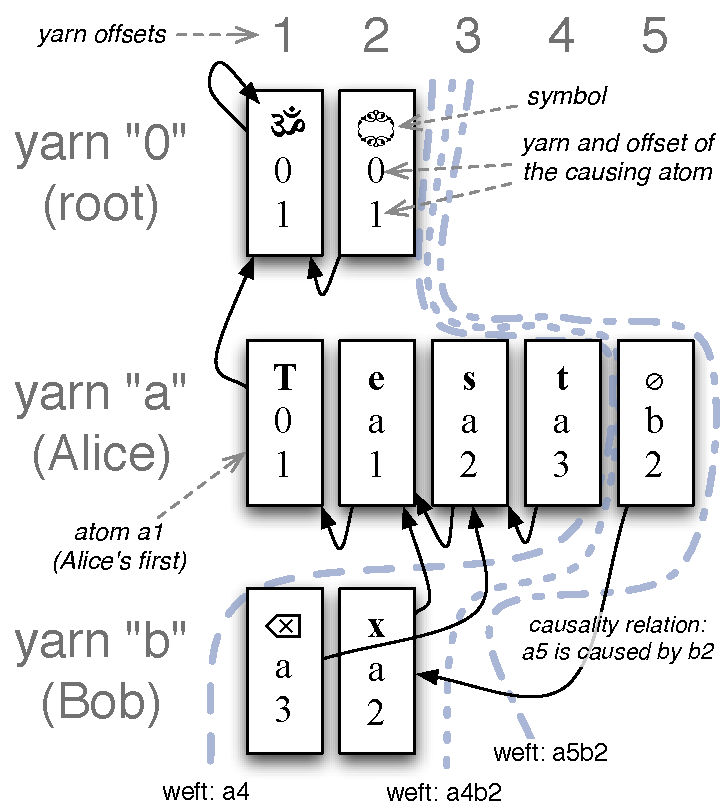
\includegraphics[width=0.48\textwidth]{feedsnweaves.pdf}
\caption{Yarns, wefts, weaves and text: Alice writes ``Test'', Bob corrects that to ``Text'', Alice saves the state. \label{fig:ds} }
~\\
\begin{tabular}{|c|c|c|l|}
\hline
{\tt weft2} & {\tt weave1} & {\tt text1} & comment\\
\hline
a4 & \aum Test{\eoa} & Test & Alice typed in ``Test'' \\
a4b2 & {\aum}Texs{\bsp}t{\eoa} & Text & Bob: ``Test''$\to$``Text'' \\
a5b2 & {\aum}Tex{\zero}s{\bsp}t{\eoa} & Text & Alice: save \\
\hline
\end{tabular}
\caption{Weft-weave-text correspondence for Fig.~\ref{fig:ds} \label{fig:wwt}}
\begin{tabular}{|c|c|c|c|c|c|}
\hline
form & {\tt atom1} & {\tt atom3} & {\tt atom3c} & {\tt atom5} & {\tt atom5c} \\
\hline
value & x & xb2 & xa2 & xb2a2 & xa2b2 \\
\hline
\end{tabular}
\caption {The ``x'' atom of Fig.~\ref{fig:ds} in different forms. \label{fig:forms}}
\end{figure}

The second basic data structure is a \emph{weft}, which is effectively a revision's identifier.
A {\tt weft2} consists of (yarn id; last symbol id) pairs, and points at the revision when those yarns were that long. 
In some sense, a weft is drawn across the yarns, hence the name.
A \emph{closed} weft is a weft unchanged by transitive closure, i.e. inclusion of all the recursive dependencies caused by yarn-to-yarn references.
The {\tt weft1} format is more condensed: it only includes last symbol ids, sorted according to the alphanumeric ordering of their yarn URLs.
%As the yarn list may extend over time (new authors join), the particular subset of mentioned yarns is defined by the length of {\tt weft1}.
Wefts are essentially vector clocks, see Sec.~\ref{sec:lamport}.

The causality relation forms a tree of atoms.
To give that tree a simpler single-root form we define zero state of any text to consist of two special symbols: start (the root) and end, designated as \aum ~and \eoa.
Any actual symbols are between those two.
In case a text was uninterruptedly typed, its causal tree degenerates into a mostly-chain, except for the \eoa ~symbol.
In either case, depth-first preorder traversal of the tree produces the text.
A closed weft cuts a rooted subtree out of the whole tree; that subtree represents a revision.
A causal tree grows in a very natural way, by forking and growing branches.
To represent atom deletion in the same fork-and-grow way, deleted atoms are not removed form the tree, but followed by backspace atoms, designated \bsp. 
Undeletion is similarly expressed as a special atom \cnc, see Sec.~\ref{sec:undo} for in-depth discussion of deletion/undeletion.
Another special atom \zero ~does nothing but signal awareness, i.e. that the author was aware of the causing atom.

The third basic data structure we use is the aforementioned \emph{weave}, normally {\tt weave5c}, which consists of all the symbols that ever existed, in order. 
Past or present revisions of a text are derived from its weave given a weft (see Fig.~\ref{fig:ds}).
All special symbols are included into the weave, but they are never shown in the resulting text, hence they cannot cause any atoms, with two exceptions: (1) \aum ~causes atoms that are inserted in the beginning of the text and (2) \zero could be caused by anything.
All modifications and transformations of a weave are done by regular expressions, while those regular expressions are often produced by other regular expressions.
The intricate dynamics of the process is considered in greater detail in the Section~\ref{sec:algos}.


\subsection {Sibling ordering}  \label{sec:siblord}

Causality creates a partial order, so it cannot directly order atoms totally into a text.
Namely, it omits ordering of siblings; in case two symbols were inserted after the same parent symbol, their causal order is undefined.
For example, the first symbol of a text is a child to \aum ~and a sibling to \eoa.
Let's define a specialization of the causal ordering to resolve the issue.

An atom $a$ is \emph{aware} of atom $b$ if $a$ is caused by $b$ or $a$ appears later in the same yarn as $b$ or there is a chain of those two relations connecting $a$ to $b$ through some intermediary atoms.
Informally, awareness means that at the time of insertion the author of $a$ knew $b$ existed. 
Each atom is aware of some (rooted) causal subtree, which is effectively a revision; that subtree may be described by a weft; let's name it awareness weft of the atom.
The awareness relation is irreflexive, asymmetric, transitive.

%once $a$ is caused by $b$, $a$ is certainly aware of $b$,
The awareness order is  defined as a preorder depth-first traversal of the causal tree, where aware (i.e. yonger) siblings are traversed first, e.g. the first symbol of the text goes before \eoa.
In many cases, awareness should be manifested manually.
Suppose, an author is inserting a symbol $a$ after a symbol $b$ which already has a child $c$, and the author's awareness of $c$ cannot be derived from the existing context.
Then, the author (effectively, the program) is supposed to first insert \zero ~after $c$ to signal awareness and thus to ensure the correct order of siblings.

The resulting ordering is still partial, as the authors may be unaware of each other doing concurrent changes, so the awareness relation still might be undefined for some siblings.
Thus, we finally introduce the total order which, be it introduced earlier, might have caused confusion.
The \emph{weft order} assumes that all atoms are ordered in accordance with depth-first preorder traversal of the causal tree, while siblings are traversed in the descending  alphanumeric order of their awareness {\tt weft1}.
This is a specialization of the awareness order, because awareness is transitive and, correspondingly, if $a$ is aware of $b$, then $\tt weft1(a) > weft1(b)$.
The inequality is strict because two symbols cannot be aware of each other (circular dependency), so their wefts surely differ.

While weft lengths may grow with the time as more authors join, the relative alphanumeric order of two {\tt weft1}s never flips.
Assuming that we compared those two wefts at a moment when their lengths were $l$, then arrival of additional $k$ coauthors will extend those wefts to the size of $l+k$ symbols.
Still, the extension is done by inserting zero symbols at exactly the same positions, corresponding to the positions of URLs of the newcomer authors in an alphabetically sorted list of yarn URLs.
In both wefts, all the newcomer's positions have equal zero values, so they do not affect the ordering.
Relativistic effects are prevented by the fact that awareness weft does not depend on the observer.
Hence, the awareness weft order is same for all observers and never flips. q.e.d.

Any changes to the text are expressed as new branches  of the causal tree; any concurrent changes (i.e. branches) are unambiguously merged and the resulting text is defined by the causal/awareness/weft order.
The model satisfies the CCI requirements.
Indeed, the causality preservation is achieved by adding changes in their awareness order.
Convergence is clear, because given the same set of atoms, peers will order them the same way, thus converging to the same state of the text.
Intention preservation is achieved by precisely identifying the place of application for every atomic operation.

The described formal system is based on simple definitions and, in most cases, it is easily implementable with regular expressions.
For example, an operation of removing every symbol followed by a backspace is just trivial.
That cannot be said about the ordering of unaware siblings; that case consumes some effort (see Sec.~\ref{sec:unre}).
The situation of two symbols being concurrently inserted at the same position in the text might not be that typical.
Still, it is important to hold the convergence requirement without any resort to central coordinating entities. 
%Namely, that all distributed replicas of a text must converge
%to the same state, if supplied with the same set of changes
%(atoms), independently of the order of arrival.
To ease the implementation of that case, I will prove
a small lemma. It will also shed more light on the
correspondence between the causal order and the order of atoms
in a weave.
First of all, a causal subtree rooted at some atom occupies
a solid interval in the weave; that is just a feature of
depth-first traversal. Let's call it a causal block.
A causal block starts with its root atom; the rest is
a sequence of zero or more causal blocks of its children.
The question is: how will we locate the end of a causality
block?
\begin{lemma} A causal block rooted at $r \ne$ \aum ~lasts till
the first atom $b$, whose parent is not $r$ but an atom
$r$ is aware of (exclusively):  $cblock(r) = [r,b)$. \label{lemma:1}
\end{lemma} 
\begin{proof}
$b$ is the first element to the right from the causal
block of $r$; $b$ surely exists. Parent of $b$ is an atom $p$,
which resides in the weave somewhere to the left from $b$.
$p \notin [r,b)$, because otherwise $b$ would also belong
to the causal block of $r$, contradiction.
Then, $p$ is to the left from $r$. Consequently, $r$ belongs
to the causal block of $p$, $r \in cblock(p)$, because
causal blocks are solid intervals and both $p$ and $b$
belong to $cblock(p)$. All atoms within a causal block are
immediately or transitively caused by its root,
ergo $r$ is aware of $p$. At the same time, no atom
within $cblock(r)$ has a parent $r$ is aware of, unless
that parent is $r$, because $r$ cannot be aware of the
atoms it caused.
\end{proof}


\section{Implementation}	   \label{sec:algos}

Low-level programming languages, such as C, allow to implement the  causal trees (CT) model directly, according to the definitions.
High-level languages, such as JavaScript, will have problems processing a causal tree where every character is an object.
That necessitates the regex implementation.
Implementing the CT model in regular expressions consumes some effort; fluency in Perl-compatible regular expression dialect (PCRE) is of great help when reading this Section. 
The number of formats and transformations employed in the causal tree model is quite high (see Fig.~\ref{fig:ops} for a general overview); but, most of transformations are implemented with a couple of regular expressions. 
For easier narration, this section will describe a typical workflow loosely based on the scenario of collaborative text authoring by several users connected to a single server.

\begin{figure}[t] \label{fig:ops}
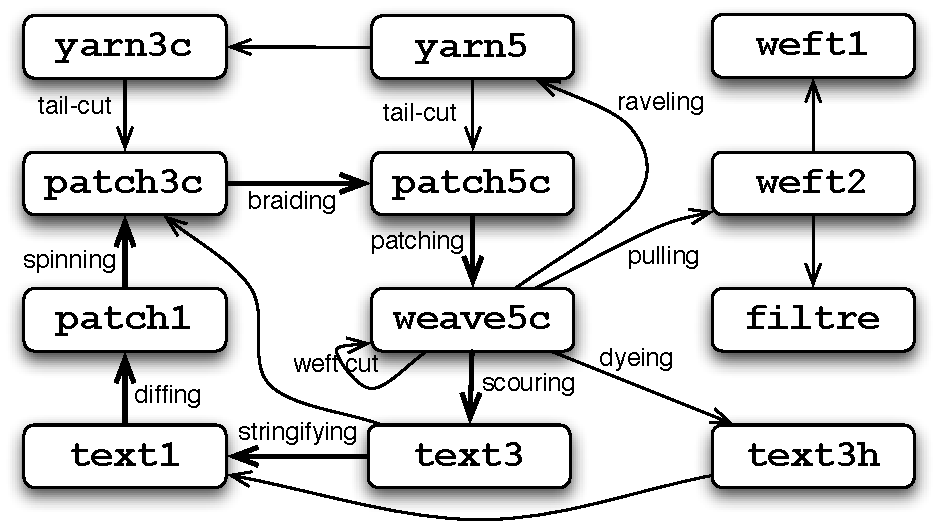
\includegraphics[width=0.48\textwidth]{operations.pdf}
\caption{Causal model formats, operations and dependencies.} \label{fig:ops}
\end{figure}

\subsection{Main loop}

The central format of the model is {\tt weave5c}, a weave where each atom is represented by its symbol, then two-char id of the causing atom, then two-char id of the atom itself, five chars total (see~Fig.~\ref{fig:forms}).
Weave might be transformed into {\tt text3} by \emph{scouring}: removing all the deleted atoms and all the special symbols from the weave: \\
{\small \verb`s/(...(..))(`\bsp\verb`\2..)+|[`\bsp\zero\verb`].{4}|.0.0.|(.)..(..)/$4$5/g`}
\footnote{Some regexes are simplified without loss of meaning. It is necessary for the ease of understanding, as PCRE is an etalon of ``write-only language''. This one ignores \cnc.}\\
The expression filters out any symbols that were deleted i.e. those that caused (are immediately followed by) an \bsp ~atom.
Out of the atom's 5c-form, only the symbol and its id are taken, thus the output is a 3-form.
{\tt text3} might be trivially \emph{stringified} into {\tt text1}, i.e. the text itself: {\small \verb`s/(.)../$1/g`}.

The text is then put into the editor; a user makes some changes.
Those changes might be tracked either by listening to  basic events or by comparing text snapshots using either the diff algorithm or heuristics.
The result is a chain of {\tt patch1} substrings corresponding to inserted and removed spans of the text; their offsets at the original text are known.
That allows to check {\tt text3} for atom ids corresponding to the change: either attachment points for insertions or sets of removed ids for deletions.
That allows to spin {\tt patch3} and further to braid a {\tt patch5c}, which contains all the inserted atoms in the 5c-form. 

{\tt patch5c} is then distributed to other users. Once it arrives, it should be integrated into their weaves.
First, it is split into causal blocks; one block is typically a causal chain of atoms corresponding to a period of uninterrupted typing.
A block has a single attachment point in the causal tree and might be inserted into the weave as a substring.
Its insertion point is just after the causing atom of the block's head/root atom, unless there is the case of unaware siblings which is addressed in Sec.~\ref{sec:unre}). Here I'll only add a safeguard by checking that the head atom is aware of the current right neighbor of its causing atom: \\
{\small \verb`s/^((?:.{5})*?)(...$C([`\bsp\cnc\verb`]$C..)*)(?=...($F))/$1$2$P/`}\\
This regex clearly needs explanation.
First of all, the regex is anchored to the beginning of the string to ensure it always matches with $\times 5$ offset and never across 5-form's atom boundaries.
Second, the regex is composed using three variables: \verb+$C, $F, $P+.
~\verb+$C+ is the atom id of the head's causing atom; \verb+$P+ is the {\tt patch5} itself; \verb+$F+ is an awareness {\tt filtre} of the head atom.
Filtre stands for ``filtering regular exppression''; {\tt filtres} are produced from {\tt weft2} by another regex, e.g. {\tt filtre('a2b4') = 'a[0-2]|b[0-4]'}.
A {\tt filtre} matches two-char atom ids that fall within the causal subtree cut by the {\tt weft2}.
Another common use for {\tt filtre} is to obtain a historical revision of a weave:  {\small \verb`s/(...($F))|.{5}/$1/g`}, which in turn may be scoured to get a historical revision of the text.
In the case of patching, we produce a {\tt filtre} out of the head symbol's awareness {\tt weft2} just to ensure the author of the head symbol was aware of the symbol to the right (no unaware siblings).

\subsection{Unaware siblings} \label{sec:unre}

Well, what if unaware siblings are introduced by other users, so the first method of patching fails?
This is exactly the situation to apply Lemma~\ref{lemma:1}. 
We single out the causality block of the heads's causing symbol, then we split it into causality blocks of the head's siblings, then we insert our block between its sibling causality blocks, according to the {\tt weft1} ordering (see Sec.~\ref{sec:siblord}).
The implementation of this case is less straightforward.
While still relying on regular expressions, it involves some ``manual'' work and, most importantly, the costly operation of \emph{pulling} (awareness weft derivation), which does several passes of the weave (see Sec.~ref{sec:pulling}).
The assumption is that concurrent insertion of symbols at the same position in the text is a rare event, so this non-trivial machinery will be invoked ``once a year''.
It should be noted that the simpler no-unaware-siblings patching algorithm employs awareness wefts as well.
Luckily, in that case wefts might be cached and incrementally updated due to append-only nature of yarns, so the costly recalculation is unnecessary.

\subsection{Pulling} \label{sec:pulling}

The operation of \emph{pulling} derives the awareness weft given an atom.
As an atom id is a trivial {\tt weft2}, pulling might be seen as transitive closure of the awareness relation.
Technically, pulling is a cycle of (a) extracting all atoms from a weave that fall under a weft and (b) using their ids to build the next iteration of the weft.
A string of concatenated ids is technically a weft, but it has lots of redundancy.
Such watery wefts are \emph{dried} into a non-redundant form by a reverse filtre that matches everything but the latest id in every yarn:
{\tt revfiltre('a1a4b2') = \verb+/a[^1-∞]|a[^4-∞]|b[^2-∞]/+}.\\
Once two consecutive iterations produce the same weft, the closure has converged.
Making numerous passes of the complete weave might be costly.
For efficiency reasons, pulling is done using a condensed form of a weave named {\tt deps4}; it contains only (id; causing id) pairs for the atoms that reference other yarns.
If an atom is caused by another atom on the same yarn, it does not affect the result of pulling. 


\subsection{Undo}	\label{sec:undo}

The undo function boils down to deleting all insertions and cancelling all deletions that happened after some recent weft.
The cancelling is done by the \cnc ~symbol, which is a ``deletion for deletions''.
The introduction of the symbol is mostly a technical optimization to allow for bulk processing of deletions and undeletions. 
(Differently from insertions, \bsp ~and \cnc ~do not form causal chains naturally and processing a thousand of \bsp ~one by one might be time-consuming.)
\cnc ~recovers its causing symbol, by cancelling all deletions it is aware of.
In general, the regex implementation employs several shortcuts to improve performance.
It is good as long as final result (the text) matches the definitions of Sec.~\ref{sec:textile}.
Special symbols are most heavily ``shortcut'' as they do not show up in the resulting text.
As an extreme example, \zero ~does not affect any operation but the pulling, and pulling does not depend on atom order.
So, just to get \zero's out of the way, they are appended to a weave just after \eoa.
All \bsp ~and \cnc ~stick to their causes as (a) they interact with their cause only, (b) they cause nothing but \zero ~and (c) their precise order is irrelevant.
All \cnc ~prepend every \bsp ~they cancel; thus, a {\tt weave5c} might have  several copies of a single \cnc, in case it cancelled multiple \bsp.
Another bulk-processing shortcut is that under certain conditions spans of \bsp ~and \cnc ~may share the id of the head symbol.
%They have no children, so their actual id is not that useful.
As we may see, the difference between theory and practice truly exists in practice.

\subsection{Misc operations}

So, we went through the full cycle: from a weave to a text
to a patch and back to the weave. Other operations are less
critical for the understanding of the model. For example, the
operation of \emph{dyeing} derives a {\tt text3h}, which is a
``painted'' text in a special 3-form showing the difference
between two revisions of a text. Namely, instead of the standard
(yarn id; symbol id) pair, a symbol is followed by a pair
of yarn ids: one for a yarn that inserted that atom,
another for a yarn that removed that atom. If no such
change happened between the two revisions, then id is null.
The {\tt text3h} string may then be transformed into
highlighted text or HTML.

The operation of saving is only supposed to signal the author's awareness/acceptance of certain revision.
Physical ``save'' to the permanent storage happens automatically once atoms are appended to yarns and broadcasted; there is no way to revoke atoms.
Thus, save is done by  adding \zero ~atoms caused by the tail atoms of all known yarns.

A solid slice of RCS functionality is dealing with branches, i.e. parallel versions of the same text/source.
In a causal tree, branch in the RCS sense correspond to literally branches of atoms.
Those branches may be attached or detached on request. Storage wise, branches might be tails of certain yarns cut off by a weft or entire special yarns.
Branches may host parts of a text with special access rights, overlay modifications (notes, annotations, bubbles/balloons), pending/discussed draft modifications or just scratchpad remarks.
As long as the point of attachment still exists in the text, a branch might be cleanly attached.
Otherwise, it is attached ``uncleanly'' into approximately the same place.
Differently form the diff-patch paradigm, the process does not depend on mutations of the context, demands no heuristics, combinatorics or manual intervention.

To summarize, the model now implements all the basic functions of a revision control system in a simple, portable and truly decentralized way.

\section{Estimations} \label{sec:estim}

Once basic data structures and algorithms of the model are explained,
it is time to consider practical feasibility of the introduced model.
It is definitely impossible to foresee every difficulty implementors may face, so this section will focus on fundamental limitations introduced by the model itself.
Section \ref{sec:formats} addresses the limits of the atom format.
Section \ref{sec:weave-growth} analyzes weave size evolution in time, using Wikipedia articles as reference data.
Section \ref{sec:io} discusses input-output (I/O) patterns of data structures used.
Section \ref{sec:sec} applies the CT model to hierarchically structured text.

\subsection{Limits of atom-based formats} \label{sec:formats}
First source of risk is CPU time necessary to process such a fine grained change/history format.
Thanks to regular expressions, all the operations listed in Section~\ref{sec:algos} run in negligible time even on bigger texts. 
If ran within a browser, $O(N)$ regular expression passes a 1MB string in around a millisecond.
The patching operation for the case of unaware siblings may take more time, let it be 100ms, but it is supposed to be a rare ``once a year'' case.
While the overall computational cost of assembling a weave from source yarns is $O(N^{2})$, i.e. a combinatory explosion is possible, unless the weave is cached.
In the latter case, $O(N^{2})$ accumulates historically, over the years of the text's lifetime.

Another risky trick is using Unicode chars as, essentially, numbers.
In fact, common regular expression engines reliably support only the first 50,000 code points or, more precisely, the $[U+0,U+D800)$ interval. 
In case a single author generates more than 50K of symbols, that author should be assigned an additional yarn id.
In total, the capacity of this numbering system limits text size to $2,5\times10^9$ symbols, which is more than enough (three volumes of ``War and Peace'' in Russian take 2,56MB in UTF-8). 
The 50,000 code points limitation also limits the number of yarns and, correspondingly, coauthors of a single document.
Practically, it is hardly a problem, as even the most popular project, namely Wikipedia, has only three articles with an author count above $2^{15}$: the Introduction, the Sandbox and the Archive of the Sandbox, i.e. pages every new user predictably bumps into.
Excluding the exercise, complaint and similar pages, the topmost ``real'' page has an author count of 13680 as of the 2009-08-16 snapshot.
That is the ``George W. Bush'' article and the reasons for the high author count are likely to be similar to the Sandbox case.
In case CT will be used for crowd-sourcing a world population census or similar purpose, there are three possible workarounds. Those are: (a) use two Unicode chars instead of one; (b) use regex engines that support $2^{32}$ character range or (c) split giant texts into smaller texts or sections (see Sec.~\ref{sec:sec}).

\subsection{Weave growth}	\label{sec:weave-growth}

The size of a text is not of big concern, as texts are small in general: the mass of Web traffic is dominated by images, not to mention video content.
The entire Web in text-only indexed form fits in a single NAS server~\footnote{According to my own experience of work in a Web search company and also some reports from inside Google.}; what actually makes web search companies to build giant facilities is the volume of simultaneous search requests.
But a weave holds the entire text's mutation history, so it may be substantially bigger than the plain text itself.
Although, for practical everyday use, full weaves are not necessary, as the user is more likely to be interested in the changes since the last visit, not the full mutation history.
Thus, some distilled version of a weave may be used, long-dead parts being {\tt filtre}d out.
Another general consideration is that the amount of processed information (think of the Web) tends to grow exponentially. Due to $\int e^{cx}dx \sim e^{cx}$, the mass of the last revision is likely to differ from the mass of the full history (i.e. weave) just by some factor.
As the saying goes, ``devil is in the details'', so let's consider the actual numbers.

\begin{figure} 
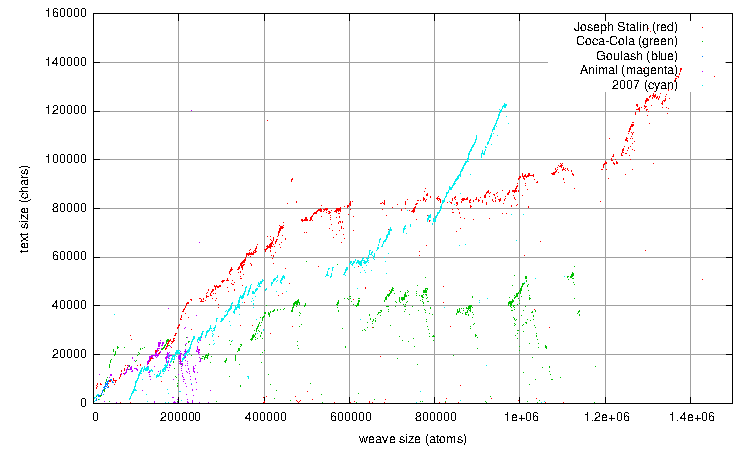
\includegraphics[width=0.48\textwidth]{weave-growth.pdf}
\caption{Weave size evolution experiments.} \label{fig:weave}
\end{figure}
\begin{figure} 
\resizebox{0.48\textwidth}{!} {
\begin{tabular}{|c|r|r|r|r|r|r|}
\hline
Article & snapsh. & .gz & .7z & {\tt weave5c} & {\tt text1} & git \\
\hline
Coca-Cola& 254Mb &78.4Mb & 482Kb & 1.13Ma & 52Kc & 9.25Mb\\
J. Stalin&754Mb& 281Mb&891Kb& 1.38Ma&137Kc& 10.6Mb\\
Goulash&2.2Mb&45Kb&26Kb&46Ka&8.6Kc& 348Kb\\
Animal & 69.9Mb & 1.1Mb & 252Kb & 254Ka & 28Kc & 3.45Mb\\
2007 & 609Mb & 191Mb & 782Kb & 967Ka & 122Kc & 10Mb\\
\hline
\end{tabular}
}
\caption{Space consumed by full-history storage in misc formats; postfix ``b'' stands for bytes, ``c'' for Unicode chars (1-2 bytes, depending on charset and encoding), ``a'' for 5-form atoms (5-10 bytes).} \label{fig:sizes} % Megabytes are decimal.
\end{figure}

To estimate growth dynamics of a weave, I plotted weave size evolution for two popular Wikipedia pages: ``Coca-Cola'' and ``Joseph Stalin''.
Weaves were derived from the full history dump dated January 2008 (the last successful one for enwiki).
The results are shown at Fig.~\ref{fig:weave}.
Vandalism was intentionally filtered out as it specifically inflates size of a weave (the entire text is deleted, then recovered back).
Namely, all changes that were rolled back within 20 revisions were  not counted.
I was checking for pairs of identical revisions to declare a rollback, so some vandalism acts were left undetected.
I assume that large gaps in the graph correspond exactly to undetected vandalism cases (weave size increased abruptly, text size stayed in place).
Still, that simple criteria provided a clear enough general picture.
During periods of unconstrained growth, weave size grows (roughly) linearly with the number of edits, as well as the article size.
But, there is also editorial pressure that tries to keep article size within bounds. Sometimes, an article gets refactored and shrinks.
Fortunately, drawing a line between cases of vandalism, edit warring, article refactoring and well-intentioned edits is out of scope of this article.

What is relevant for us is the general correspondence between space requirements of different text storage formats.
I've conducted an experiment, comparing history sizes of several Wikipedia articles kept in six formats: bare snapshots, gzip and 7zip of snapshots, {\tt weave5c}, plain text of the last revision (no history) and a git repository keeping the entire history, see Fig.~\ref{fig:sizes}.
As a rule of a thumb, \emph{full} weave size may be estimated as x100 the plain text size.
Mass of a pre-filtered weave is likely be around text size times 5 or 10, depending on charset/encoding, which factor is defined by the form-5 overhead.
Interestingly enough, a gzip of snapshots is far worse than an uncompressed weave.
A 7zip archive is better off, its main shortcoming being high CPU consumption (it took around 20 seconds to unpack some of the articles).
Space efficiency of {\tt weave5c} as a versioned text format is comparable to the space efficiency of the git RCS repository storing the same page history (measured immediately after \verb+git gc+, i.e. compression and garbage collection).
As a summary, weave is effective as a server-side versioned text format. 
For the client side, a weave better be prefiltered to keep only those changes of interest.

\subsection{I/O patterns}	\label{sec:io}

Finally, as we talk about data storage formats, it is definitely useful to consider their I/O patterns.
A weave is convenient for reading and processing, which is done in sequential passes.
It is much less convenient for writing, as it needs to be overwritten entirely after any modification.
A yarn is exactly the opposite: it is append-only, so writing is cheap, while reading and weaving together many yarns is both CPU and I/O consuming operation.
In practical scenarios, mixed solutions are better.
As an example, consider the {\tt weave5c+patch5c+text1} set.
Read-only clients may be served with {\tt text1}.
All ongoing modifications might be appended to {\tt patch5c}, which thus acts as a write cache.
The {\tt weave5c}, once read from the disk, should be immediately  updated with the {\tt patch5c}.
Once {\tt patch5c} becomes too big, the weave might be overwritten with its current version, {\tt patch5c} is thus emptied.
Other mixes are also possible, depending on trade-offs.
For native (non-regex) implementations, tradeoffs might be different; e.g. a {\tt weave5} might be assembled from a set of {\tt yarn3c} in linear time; as yarns are append-only they are also perfectly cacheable, etc etc.

\subsection{Sectioned model}	\label{sec:sec}

The causal trees model exclusively considers plain/flat text; formatted text is often modeled as a tree structure, e.g. HTML's Document Object Model (DOM)~\cite{dom}.
I will sketchily address this concern.~\footnote{My understanding of what should and what should not be done here is based on the experience of building a chain of prototypes over the past years~\cite{www06,csr07,wikisym08}.} 

While DOM imposes hierarchical structure on formatted text, the text per se was not historically considered hierarchical, except probably for its bigger units, i.e. \emph{sections}. 
Remember LaTeX, the RFC text format, the wikitext or even the early pre-DOM HTML: the text is considered to be a flow of words and markup elements, the only hierarchically structured parts are sections/subsections.
Even browsers, as a matter of fact, start parsing with the ``tag soup'' model, later applying some heuristics to transform it into an orderly tree. 

Note the open possibility to handle units of text hierarchical structure (sections) separately.
While each section might be considered flat in the pre-DOM HTML sense, different sections might reference each other through transclusion links thus forming a hierarchical structure.
Each section has its own weave; as a weave is just a string, the resulting data structure is simple enough.
As a result, we have a digraph of sections; that keeps the complexities of the document's hierarchy and revision control orthogonal. 

The sectioned structure allows to preserve histories once a section is moved within a document or even between documents.
With equal ease, it allows to prune old history once an article is refactored.
Removed sections are still mentioned in histories of their parent sections, so historical revisions of the whole document can be recovered. At the same time, long-dead parts do not clutter the weaves currently in use.
Last but not least, the sectioned structure allows to relax the 50,000 authors limitation: a single section might not have 50K symbols, not to mention authors.

Back to HTML, the correct XHTML structure cannot be guaranteed when merging concurrent modifications: for example, two overlapping tag ranges cannot be merged correctly in the general case, e.g. 
{\small \verb+<i>Quick <b>brown</i> fox</b>+. }\\
That of course returns us to the tag soup situation; but that is the state of the things anyway and  browsers are good in dealing with it. 
Once the correct hierarchical structure of the text is ensured by the structure of (isolated) sections, best-effort merge of decorative tags within sections may be offloaded to the browser.
In either case, this alternative seems more practical than distributed real-time revision control of DOM trees (see Sec.~\ref{sec:waveot}).


\section{Parallels and reflections} \label{sec:reflections}

Throughout the paper, our model was compared to the classic
diff/patch/snapshot revision control paradigm. 
...
reuses
combines atom ids and vector clocks in a practical regex-processible form and  carefully ... awareness order
...
It certainly makes
sense to put it in a broader context to uncover diverse
similarities and dependencies.

\subsection{Operational Transformation} \label{sec:ot}

First of all, the causal model fulfills three requirements of OT.
Causality preservation holds
by design, as an atom is never introduced to the weave before all
any of the atoms it is aware of.
Convergence is insured as the order of atoms in a weave does
not depend on the order of arrival. Intention
preservation, in the sense of applying changes to a wrong position
in the text, is trivially solved: the logic is not positional.
In general, introducing unique atom identifiers and putting
atoms orderly into a tree removed all the arcane complexity
of position-dependent operations and transformations.

Differently from operational transformation schemes, causal trees
absolutely lack the transformation aspect: atomic operations
stay intact and interact in simple predictable ways. That brings
it closer to the WOOT~\cite{woot} transformationless OT scheme
that also abandons positional logic in favor of unique atom
identification. While WOOT records both neighbors of a newly
introduced atom, CT records just one (the ``cause''). 
In some situations, indeed, CT has to mention the second
neighbor using the \zero ~atom, but that is an exception.
WOOT avoided using vector clocks, based on the assumption that
the size of a vector is proportional to the total number of
participants. But in the scope of a single page or a
section the number of editors is manageable; vector clocks
(wefts) also turn to be quite handy as revision identifiers.
As well, CT has some similarities to another post-OT system
Logoot~\cite{logoot}. Logoot's list-identifiers can be compared
to concatenations of CT ids along the path from the root to 
the atom. In CT, this structure is used implicitly.
Logoot's arguments against thombstones are much less relevant
for symbol-based revision control (as opposed to line-based).

\subsection{Fidge-Lamport vector clocks} \label{sec:lamport}

The causal tree model perfectly matches entities of the
Lamport - Fidge~\cite{lamport,fidge} vector/logical clocks model.
Namely, yarn
corresponds to a process, foreign causality relations - to
messages, yarn offsets to local logical clocks and wefts to
vector clocks. 
Awareness order follows the lines of Lamport's synchronized
logical timestamps. The weft order is similar to Fidge's vector
clock ordering, but there are no strict equivalence here.

\subsection{Xanadu}

There are some parallels between causal trees and the historical
Xanadu hypertext model. The spirit of Xanadu is to keep all the
versions of all texts at the same time, by clearly separating the
original input from the actual revisions of the text. Very similar 
approach is seen in causal trees: primary input is put into yarns
while all the actual revisions are subsequences of the weave.
The implementation method is different.

\subsection{Wikipedia}

Currently, Wikipedia faces scaling problems~\cite{no-singularity,wp-decay};
nature of those problems is quite complicated and cannot be fully
covered in this article. Some research effort was put into
engineering Wikipedia decentralization based on Distributed
Hash Tables (DHTs, ~\cite{urdaneta}). That is merely a
technical decentralization that addresses possible funding
shortages. Another side of the problem is social decentralization.
How to prevent turf wars and contributor alienation? Is it
possible to create multiple competing pedias? How could we
possible test novel forms of contributor organization and
incentivization? Will the inclusionist approach work, i.e.
could we use Wikipedia for specialized knowledge?

My honest belief is that decent decentralized revision control
is absolutely necessary just to start thinking about those
questions. Eventually, decentralized version control with
easy forking and easy merge of branches may lead towards the
vision that Linus Torvalds has explained as ``crosspollination
and natural selection''~\cite{linus-pollinates}
in application to the Linux development;
currently, those ideas are manifested in the design of the git RCS.
Unfortunately, the git is not Web-ready. It is precisely fit
for its current purpose and it was never intended to be run
in a browser or to be simple enough, etc.

\subsection{Google Wave}  \label{sec:waveot}

Google Wave relied on a flavor of Operational Transformation for
real-time version control. The enhanced OT flavor is supposed to
handle both plain text and tree-like XML DOM structures.
Informally, the main problem of the resulting technology is that
its complexity is OT complexity \emph{times} XML complexity. 
The authors even had to enrich XML with additional entities 
named ``annotations'' to make it suitable for their needs.
There are 15 sorts of different mutation operations used in Wave
OT, some as opaque as ``delete anti-element end''~\cite{waveot}.
Theoretically, the potential for unexpected feature interactions
tends to grow combinatorially with the number of primitives.
In practice, the overcomplication resulted in numerous bugs and
slow unresponsive user interface~\cite{own-experience}.
According to an insider~\cite{gerasimov}, in 6 months since the
projects's launch the possibility of working with partial
histories is not  implemented yet; pages are bootstrapped with
their complete histories. Compare that to the ease of applying
a filtre to a weave in the CT model.

\subsection{Source Code Management}

empower the user ...
The ability to express branches (in the RCS sense, i.e. parallel text versions) as bunches of causal branches (i.e. subtrees) opens some new interesting possibilities.
For example, Linux developers are familiar with ``patch sets'' -- changes to the kernel that are maintained in parallel. Similarly, it is possible to maintain ``transparent overlays'' over the text, i.e. sets of changes that may be switched on or off. These ``overlay'' changes might be stored as yarns or tails of yarns, referencing the core of ``universally accepted'' yarns one-way.
...

\section {Conclusion} \label{sec:conclusion}

While many previous revision control solutions were either
fully distributed or real-time or Web-based, the causal trees
combine all that at once. Thanks to a very simple string based
format and trivially portable regex-based algorithms, causal trees
have a good chance of making the critical step from an
application to an open format used at mass scale in highly
distributed highly heterogeneous environment, which is the Open Web.


\section{Acknowledgements}

Many thanks to Mikhail Volkov, Bram Cohen,
Alexandr Pronchenkov, Sergey Pupyrev and Jan Gerber for priceless
feedback that influenced this paper.

\bibliographystyle{plain}
\bibstyle{plain}

\bibliography{sources}

\end{document}
